\section{Grundlagen}\label{kap:grundlagen}
In diesem Kapitel werden einige Grundlagen für die in Kapitel \ref{kap:featureextraktion} diskutierten Algorithmen besprochen.
\subsection{Was sind Sensordaten}\label{kap:sensordaten}
Um Maschinen zu steuern werden oft bidirektionale Datenflüsse verwendet. 
Das Kontrollsystem gibt Anweisungen und reagiert anschließend auf das Feedback der Maschine. 
Teilweise werden auch einfache Zeitschranken als Feedback verwendet. 
Sensoren optimieren das Feedback für das Kontrollsystem. 
Um Maschinen zu überwachen, können diese Feedback- und Sensordaten verwendet werden um beispielsweise Datenabweichungen festzustellen. 
Weitere Umgebungssensoren, wie auch Kamereasysteme, Temperatur- und Kontaksensoren, bieten meist einen Informationshaltigen Datenbestand. 
Dabei können Temperaturunterschiede, Verschlusszeiten, Druckaufbauzeiten u.ä. betrachtet werden. 
Die spezielle Herausforderung bei Sensordaten ist der kontinuierliche Datenfluss. 
Bei laufender Maschine werden stetig Daten generiert sowohl bei Gut- als auch Schlechtdurchläufen. 
Die Anforderung an das Überwachungssystem ist somit die kontinuierliche Datenverarbeitung. 
Es wird von einer Livedatenanalyse gesprochen.
In der Livedatenanalyse müssen die Daten genauso schnell verarbeitet werden wie sie als Eingabe zur Verfügung stehen, damit sich kein \enquote{Datenstau} ergibt. 

\begin{center}
  -TODO- Beispieldatensatz
\end{center}

\begin{figure}
  \centering
  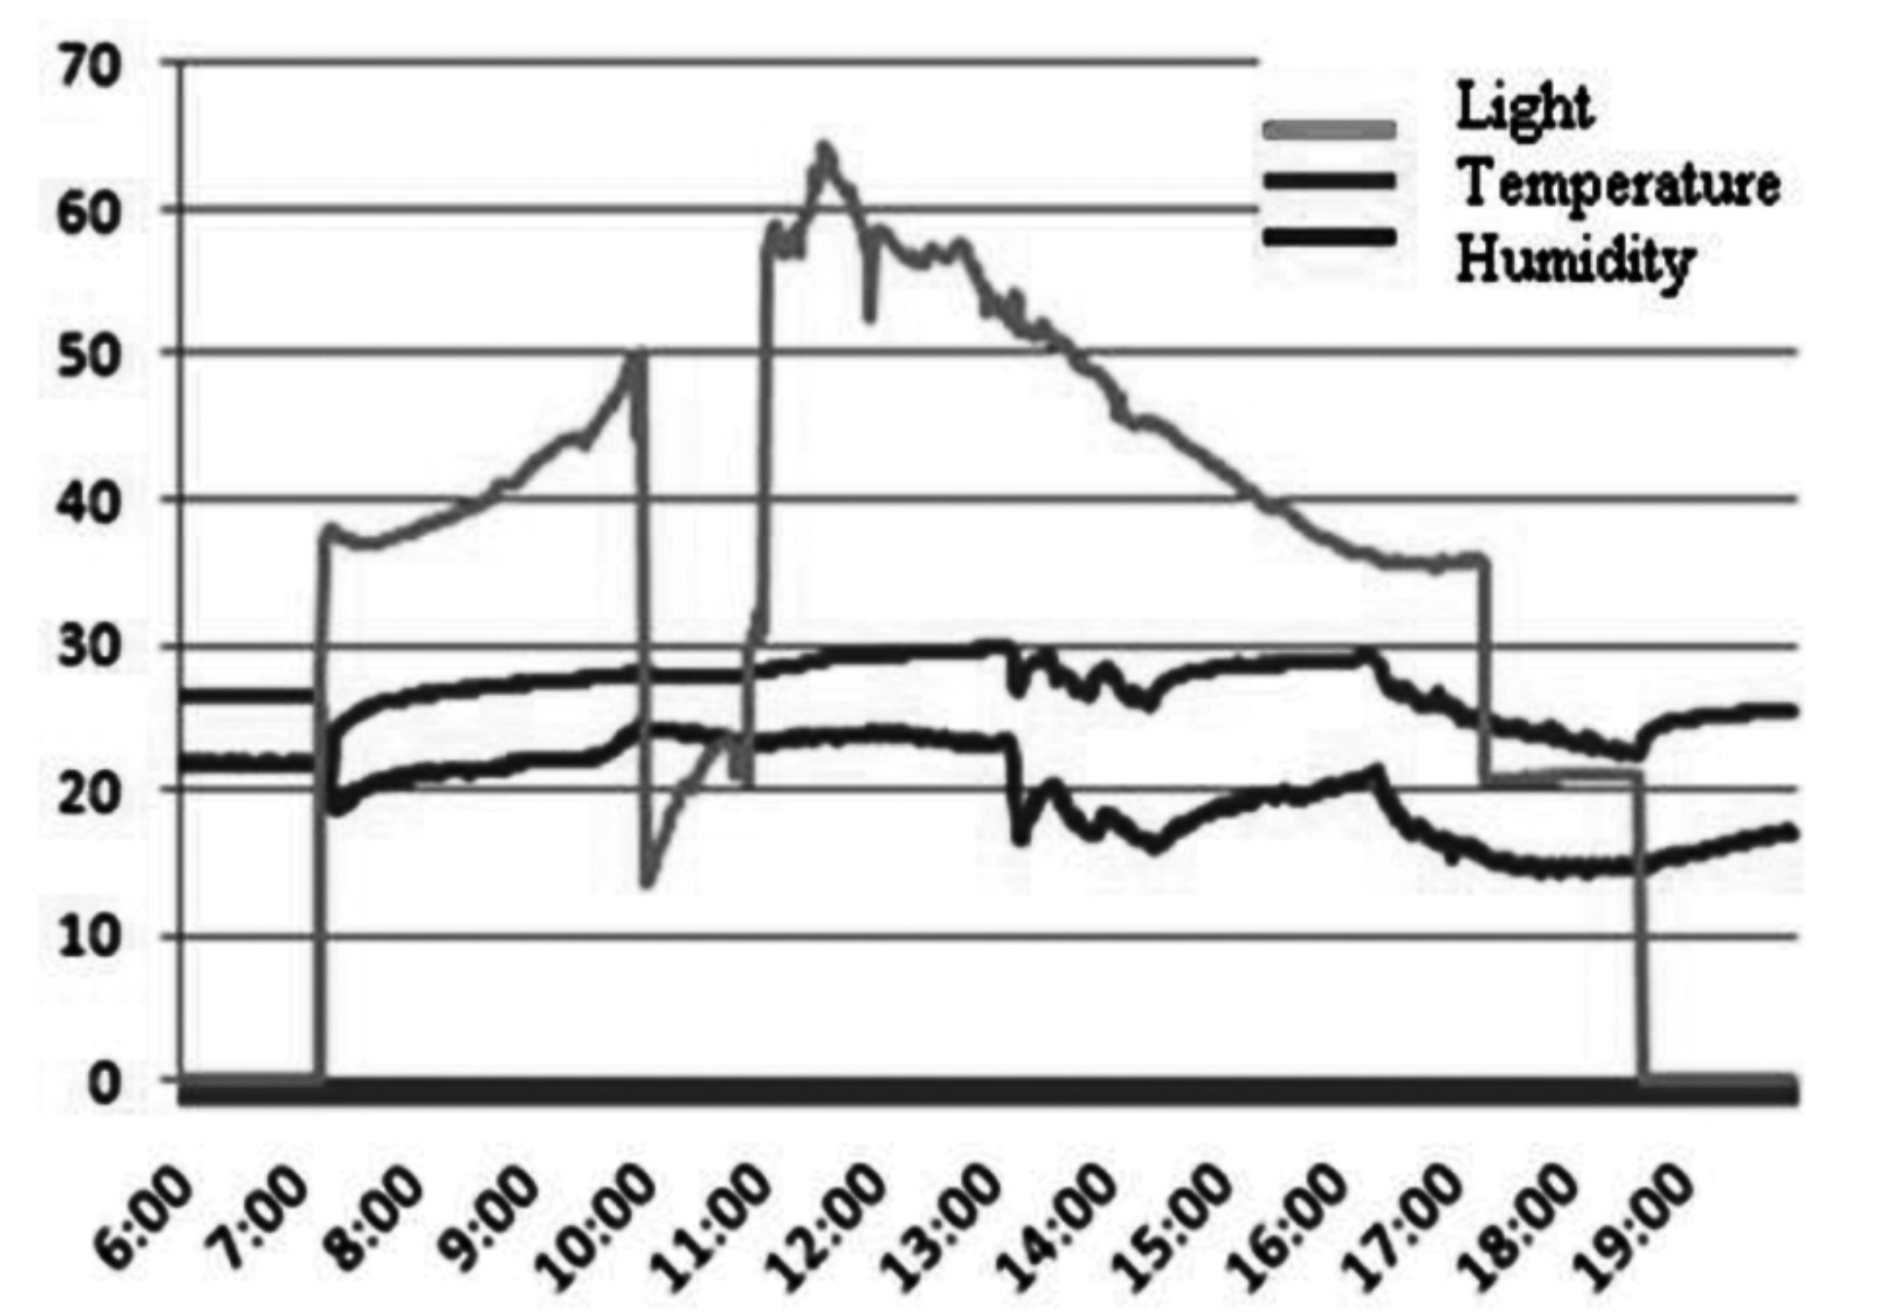
\includegraphics[width=.8\textwidth]{datasetOffice.png}
  \caption{Sensordatenabweichung anhand von Licht, Temperatur und Drucksensoren im Buro innerhalb von einem Arbeitstag~\cite{moraru2010using}}
  \label{fig:datasetoffice}
\end{figure}


Abbildung \ref{fig:datasetoffice} zeigt die Sensordatenabweichung im Büro innerhalb eines Arbeitstages. 
Zu jedem Zeitpunkt kann der Datensatz ausgewertet und differenziert werden. 
Beispielsweise unterscheiden sich die Datenwerte von 8:00 Uhr und 9:99 Uhr masgeblich an der Helligkeit. 
Mathematisch würde dieser Zeitpunkt als Vektor dargestellt werden.
\begin{equation}
  x_1 =
\begin{pmatrix}
    38\\
    20\\
    25 
\end{pmatrix}
\end{equation}
Durch die Vektordarstellung können die Datenpunkte anhand ihrer Parameter unterschieden werden. Durch betrachten von Zeitreihen, lassen sich an mehereren Tagen Muster erkennn. Solche Zeitreihendaten können Mathematisch als Matrix dargestellt werden.
\begin{equation}
  x_{1,4}
  \begin{pmatrix}
      38 & 40 & 45 & 20\\
      20 & 22 & 23 & 23\\
      25 & 28 & 29 & 29
  \end{pmatrix}
\end{equation}

Um Mathematisch mehrere Tage in einen Datensatz darzustellen erhalten wir schon Tensoren.
Schon anhand dieses simplen Beispiels wird die Datenmenge und Komplexität der Daten ersichtlich.
Algorithmen zur Livedatenanalyse solcher komoplexer Datenbestände werden in Kapitel \ref{kap:featureextraktion} besprochen.

\begin{center}
  -TODO- Es fehlt noch ein Kapitel für kurze ML einleitung. Regressionen, Klassifikationen. Und den Bezug zur Maschinenüberwachung. 
\end{center}

Speziell in der Maschinenüberwachung ist das Ziel solche Daten nicht nur im aktuellen Zeitpunkt zu bewerten, sondern eine Vorhersage zu treffen. Angenommen wir betrachten einen Datensatz zum Zeitpunkt $t_1$. Dann besteht der zu bewertender Datensatz aus einem Tupel $\tau_1=(t_1,x_1)$. Diesem Tupel wird abhängig von den verwendeten Verfahren eine Klasse $y_1$ zugewiesen~\cite{gay2013feature}. Für den Zeitraum $(t_1,...,t_n)$ mit $n \in \mathbb{N}$ erhalten wir den Datensatz 
\begin{equation}
  D=\{ (\tau_1,y_1), ... , (\tau_n,y_n) \}
  \label{equ:trainingset}
\end{equation}
Das Ziel ist das Tupel $(t_{n+1},y_{n+1})$ voherzusagen.

\subsection{Was versteht man unter Feature Extraktion}\label{kap:featureextraktionuebersicht}
In Kapitel \ref{kap:sensordaten} wurde ein Datensatz durch seine Muster und Merkmale beschrieben. Merkmale können einfache Parameter, wie Schwellwertüberschreitungen sein. In Komplexeren Datenstrukturen, können die Daten anhand von Verlaufsmustern unterschieden werden. 

Um Algorithmen zu trainieren die Daten durch diese Merkmale und Muster zu unterscheiden, gibt es zwei wesentliche herangehensweisen. Es können die Merkmale dem Algorithmus vorgegeben und auf diese Merkmale trainiert werden, oder es werden Verfahren angewendet um diese Merkmale zu extrahieren. Es ist die Rede von \enquote{Feature Extraktion}. Ein \enquote{Feature} ist eines dieser Merkmale, wodurch Daten in einem Datensatz voneinander unterschieden werden können. 

Dabei ist das Ziel die Features so zu wählen und zu parametrisieren, dass das der ermittelte Wert dem tatsächlichen Wert möglichst ähnelt. Betrachten wir die Gleichen \ref{equ:trainingset} und die daraus ermittelte Funktion $p(x_i)$, welche das Ergebnis des gewählten Algorithmus und des Trainingsdatensatzes ist. Es soll versucht werden den Fehlerunterschied

\begin{equation}
  \sigma = p(x_i)-y_i
\end{equation}

möglichst zu reduzieren~\cite{gensler2015fast}. Konkret wird meist die Summe der Quadratischefehler
\begin{equation}
  \sigma^2 = \frac{1}{N} \sum_{i=0}^{K}(p(x_i)-y_i)^2
\end{equation}
versucht zu reduzieren.

\begin{center}
  - TODO - Ein konkretes Beispiel für Feature Extraktion raussuchen und daran erkären. Es muss auch noch die Notwendigkeit und die herangehensweise von Dimensionsreduzierung erläutert werden.
\end{center}

\begin{itemize}
  \item Kurze ML einleitung mit erklärung zur Feature-Extraktion
  \item Feature extraction vs Feature selection
  \item \enquote{extrahieren von Merkmalen, wodurch die Daten in einem Datensatz voneinander unterschieden werden können}
\end{itemize}